\documentclass[12pt]{beamer}
\usepackage{../Estilos/BeamerMAF}
\usepackage[absolute, overlay]{textpos}
\usepackage{../Estilos/ColoresLatex}
\usetheme{Copenhagen}
\usecolortheme{wolverine}
%\useoutertheme{default}
\setbeamercovered{invisible}
% or whatever (possibly just delete it)
\setbeamertemplate{section in toc}[sections numbered]
\setbeamertemplate{subsection in toc}[subsections numbered]
\setbeamertemplate{subsection in toc}{\leavevmode\leftskip=3.2em\rlap{\hskip-2em\inserttocsectionnumber.\inserttocsubsectionnumber}\inserttocsubsection\par}
% \setbeamercolor{section in toc}{fg=blue}
% \setbeamercolor{subsection in toc}{fg=blue}
% \setbeamercolor{frametitle}{fg=blue}
\setbeamertemplate{caption}[numbered]

\setbeamertemplate{footline}
\beamertemplatenavigationsymbolsempty
\setbeamertemplate{headline}{}


\makeatletter
% \setbeamercolor{section in foot}{bg=gray!30, fg=black!90!orange}
% \setbeamercolor{subsection in foot}{bg=blue!30}
% \setbeamercolor{date in foot}{bg=black}
\setbeamertemplate{footline}
{
  \leavevmode%
  \hbox{%
  \begin{beamercolorbox}[wd=.333333\paperwidth,ht=2.25ex,dp=1ex,center]{section in foot}%
    \usebeamerfont{section in foot} \insertsection
  \end{beamercolorbox}%
  \begin{beamercolorbox}[wd=.333333\paperwidth,ht=2.25ex,dp=1ex,center]{subsection in foot}%
    \usebeamerfont{subsection in foot}  \insertsubsection
  \end{beamercolorbox}%
  \begin{beamercolorbox}[wd=.333333\paperwidth,ht=2.25ex,dp=1ex,right]{date in head/foot}%
    \usebeamerfont{date in head/foot} \insertshortdate{} \hspace*{2em}
    \insertframenumber{} / \inserttotalframenumber \hspace*{2ex} 
  \end{beamercolorbox}}%
  \vskip0pt%
}
\makeatother

\makeatletter
\patchcmd{\beamer@sectionintoc}{\vskip1.5em}{\vskip0.8em}{}{}
\makeatother

% %\newlength{\depthofsumsign}
% \setlength{\depthofsumsign}{\depthof{$\sum$}}
% \newcommand{\nsum}[1][1.4]{% only for \displaystyle
%     \mathop{%
%         \raisebox
%             {-#1\depthofsumsign+1\depthofsumsign}
%             {\scalebox
%                 {#1}
%                 {$\displaystyle\sum$}%
%             }
%     }
% }
% \def\scaleint#1{\vcenter{\hbox{\scaleto[3ex]{\displaystyle\int}{#1}}}}
% \def\scaleoint#1{\vcenter{\hbox{\scaleto[3ex]{\displaystyle\oint}{#1}}}}
% \def\bs{\mkern-12mu}


\setbeamercolor{section in foot}{bg=babyblue, fg=black}
\setbeamercolor{subsection in foot}{bg=blond, fg=black}


\makeatletter
\setbeamertemplate{footline}
{
\leavevmode%
\hbox{%
\begin{beamercolorbox}[wd=.333333\paperwidth,ht=2.25ex,dp=1ex,center]{section in foot}%
  \usebeamerfont{section in foot} \insertsection
\end{beamercolorbox}%
\begin{beamercolorbox}[wd=.333333\paperwidth,ht=2.25ex,dp=1ex,center]{subsection in foot}%
  \usebeamerfont{subsection in foot}  \insertsubsection
\end{beamercolorbox}%
\begin{beamercolorbox}[wd=.333333\paperwidth,ht=2.25ex,dp=1ex,right]{date in head/foot}%
  \usebeamerfont{date in head/foot} \insertshortdate{} \hspace*{1.5em}
  \insertframenumber{} / \inserttotalframenumber \hspace*{2ex} 
\end{beamercolorbox}}%
\vskip0pt%
}
\makeatother
\usefonttheme{serif}
\setbeamercolor{frametitle}{bg=champagne}
\resetcounteronoverlays{saveenumi}

\date{24 de mayo de 2022}

\title{\large{Oscilaciones en una cadena colgante}}
\subtitle{Funciones de Bessel}
\author{M. en C. Gustavo Contreras Mayén}

\begin{document}
\maketitle
\fontsize{14}{14}\selectfont
\spanishdecimal{.}

\section*{Contenido}
\frame{\frametitle{Temas a revisar} \tableofcontents[currentsection, hideallsubsections]}


%Ref.  (2018) - Oscillations of a hanging chain
\section{Planteamiento}
\frame{\tableofcontents[currentsection, hideothersubsections]}
\subsection{Enunciado del problema}

\begin{frame}
\frametitle{Planteamiento del problema}
Considera una cadena flexible uniforme (o cuerda pesada) de longitud $L$, que está fija en el extremo superior y libre en el extremo inferior.
\\
\bigskip
\pause
Dejamos que el eje $x$ sea vertical, medido desde la posición de equilibrio del extremo libre de la cadena.
\end{frame}
\begin{frame}
\frametitle{Planteamiento del problema}
La función $Y (x, t)$ es el desplazamiento horizontal de la cadena en el punto con la coordenada vertical $x$ en el tiempo $t$, el sistema se presenta en la siguiente figura.
\end{frame}
\begin{frame}
\frametitle{La cadena colgante}
\begin{figure}[H]
    \centering
    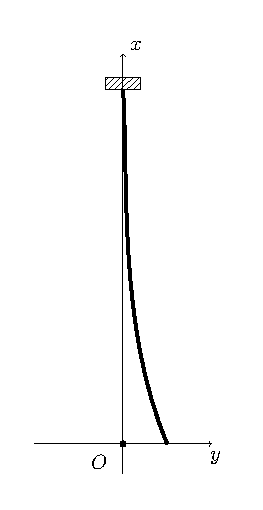
\includegraphics[scale=0.8]{Imagenes/Cadena_Oscilante_01.eps}
    %\caption{Cadena oscilante y el sistema coordenado.}
    %\label{fig:figura_cadena_inicial}
\end{figure}
\end{frame}
\begin{frame}
\frametitle{Estudiando el sistema}
Suponemos que $Y (x, t)$ es pequeña en comparación con la longitud de la cadena $L$.
\\
\bigskip
\pause
Por lo tanto, no consideramos  la diferencia entre las distancias medidas a lo largo de la cadena y las distancias medidas a lo largo del eje $x$, es decir, podemos omitir los términos:
\pause
\begin{align*}
\sqrt{x^{2} + Y^{2}} - x \thicksim \dfrac{Y^{2}}{x}
\end{align*}
\end{frame}
\begin{frame}
\frametitle{Consideraciones al problema}
Por la misma razón, podemos cancelar el desplazamiento vertical debido a las oscilaciones.
\\
\bigskip
\pause
También suponemos que el ángulo $\alpha (x)$ entre la dirección local de la cadena y el eje $x$ es pequeño, por lo tanto:
\pause
\begin{align}
\sin \alpha \approx \tan \alpha = \pdv{Y}{x}
\label{eq:ecuacion_01}
\end{align}
\end{frame}
\begin{frame}
\frametitle{Componentes de la tensión}
La componente horizontal de la fuerza neta que actúa sobre un segmento de la cadena de longitud $\Delta x$ debido a la tensión interna $T (x)$ es:
\pause
\begin{align}
\begin{aligned}[b]
T (x  + \Delta x) \, &\pdv{x} Y (x + \Delta x) - T (x) \, \pdv{x} Y (x) \\[0.5em] \pause
&\approx \pdv{x} \bigg[ T (x) \, \pdv{Y}{x}  \bigg] \, \Delta x
\end{aligned}
\label{eq:ecuacion_02}
\end{align}
\end{frame}
\begin{frame}
\frametitle{Componentes de la tensión}
\begin{figure}[H]
    \centering
    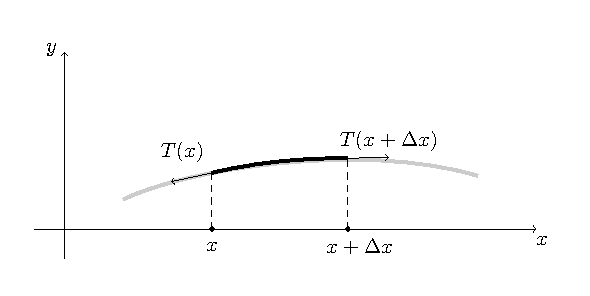
\includegraphics[scale=1.1]{Imagenes/Cadena_Oscilante_02.eps}
    %\caption{Fuerzas actuando en el elemento de la cadena.}
    \label{fig:figura_elemento_cadena}
\end{figure}
\end{frame}
\begin{frame}
\frametitle{Recupeando la ecuación de movimiento}
La segunda ley de Newton nos proporciona la ecuación de movimiento:
\pause
\begin{align}
\pdv{x} \bigg[ T (x) \pdv{Y}{x} \bigg] \, \Delta x = \rho \, \Delta x \, \pdv[2]{Y}{x}
\label{eq:ecuacion_03}
\end{align}
donde:
\pause
\setbeamercolor{item projected}{bg=yellow,fg=black}
\setbeamertemplate{enumerate items}{%
\usebeamercolor[bg]{item projected}%
\raisebox{1.5pt}{\colorbox{bg}{\color{fg}\footnotesize\insertenumlabel}}%
}
\begin{enumerate}[<+->]
\item $\rho$ es la densidad lineal de la cadena (masa por unidad de longitud).
\item $\rho \, \Delta x$  es la masa del segmento.
\item $\displaystyle \pdv[2]{Y}{x}$ es la aceleración.
\end{enumerate}
\end{frame}
\begin{frame}
\frametitle{Manejando la expresión}
Cancelando el factor común $\Delta x$ en ambos lados de la ec. (\ref{eq:ecuacion_03}), tenemos:
\pause
\begin{align}
\pdv{x} \bigg[ T (x) \pdv{Y}{x} \bigg] = \rho \, \pdv[2]{Y}{x}
\label{eq:ecuacion_04}
\end{align}
\end{frame}
\begin{frame}
\frametitle{Suponiendo oscilaciones pequeñas}
Para pequeñas oscilaciones de la cadena, cuando podemos cancelar el desplazamiento vertical debido a las oscilaciones, \pause la tensión $T (x)$ es la misma que para la cadena en reposo, \pause es decir, la tensión en el punto con la coordenada vertical $x$ es igual al peso de la parte de la cadena debajo de $x$.
\end{frame}
\begin{frame}
\frametitle{Valor de la tensión}
Por lo tanto:
\pause
\begin{align}
T = \rho \, g \, x
\label{eq:ecuacion_05}
\end{align}
donde $g$ es la aceleración debida a la gravedad.
\end{frame}
\begin{frame}
\frametitle{Revisando las CDF}
La cadena está fija en la parte superior, por lo tanto:
\pause
\begin{align}
Y (0, t) = 0
\label{eq:ecuacion_06}
\end{align}
\end{frame}
\begin{frame}
\frametitle{Desplazamiento en el otro extremo}
El desplazamiento en el extremo libre de la cadena permanece finito en todo momento, así que:
\pause
\begin{align}
\abs{Y (L, t)} < \infty
\label{eq:ecuacion_07}
\end{align}
\end{frame}

\section{Resolviendo la ecuación}
\frame{\tableofcontents[currentsection, hideothersubsections]}
\subsection{Separación de variables}

\begin{frame}
\frametitle{Ocupando la separación de variables}
Resolvemos la ecuación diferencial parcial mediante la separación de variables ec. (\ref{eq:ecuacion_03}) con las condiciones de frontera ecs. (\ref{eq:ecuacion_06}), (\ref{eq:ecuacion_07}), es decir, suponiendo que:
\pause
\begin{align}
Y (x, t) = y (x) \, u (t)
\label{eq:ecuacion_08}
\end{align}
\end{frame}
\begin{frame}
\frametitle{Manejando la expresión}
Sustituyendo la ec. (\ref{eq:ecuacion_08}) en la ec. (\ref{eq:ecuacion_04}), obtenemos:
\pause
\begin{align}
u (t) \, \dv{x} \bigg[ T (x) \, \dv{y}{x} \bigg] = \rho \, y (x) \, \dv[2]{u}{t}
\label{eq:ecuacion_09}
\end{align}
\end{frame}
\begin{frame}
\frametitle{Manejando la expresión}
Que mediante un arreglo de las funciones $u$ e $y$, se tiene:
\pause
\begin{align}
\dfrac{1}{y (x)} \, \dv{x} \bigg[ T (x) \, \dv{y}{x} \bigg] = \rho \, \dfrac{1}{u (t)} \, \dv[2]{u}{t}
\label{eq:ecuacion_10}
\end{align}
\end{frame}
\begin{frame}
\frametitle{Separando las variables}
El lado derecho de la ec. (\ref{eq:ecuacion_10}) es una función del tiempo $t$.
\\
\bigskip
\pause
El lado izquierdo es una función de $x$. \pause Los dos lados pueden ser iguales en todo momento y coordenadas solo si ambos son iguales a la misma constante.
\end{frame}
\begin{frame}
\frametitle{La constante de separación}
Como veremos en breve, esta constante debe ser real y negativa.
\\
\bigskip
\pause
De hecho, el sistema mecánico descrito por la ec. (\ref{eq:ecuacion_03}) es conservativo.
\end{frame}
\begin{frame}
\frametitle{La constante de separación}
Por lo tanto, la función $u (t)$ no puede crecer sin límite o reducirse a cero.
\\
\bigskip
\pause
Las soluciones permitidas solo son posibles para constantes de separación negativa reales.
\end{frame}
\begin{frame}
\frametitle{La constante de separación}
Denotando la constante de separación por $- \omega^{2}$, obtenemos las siguientes ecuaciones:
\pause
\begin{align}
\dfrac{1}{u (t)} \, \dv[2]{u}{t} &= - \omega^{2} \label{eq:ecuacion_11} \\[0.5em]
\dfrac{1}{y (x)} \, \dv{x} \bigg[ T (x) \, \dv{y}{x} \bigg] &= - \rho \, \omega^{2} \label{eq:ecuacion_12}
\end{align}
\end{frame}

\subsection{Las soluciones}

\begin{frame}
\frametitle{La solución $u (t)$}
La ec. (\ref{eq:ecuacion_11}) se resuelve fácilmente:
\pause
\begin{align}
\dv[2]{t} + \omega^{2} \, u (t) = 0
\label{eq:ecuacion_13}
\end{align}
\end{frame}
\begin{frame}
\frametitle{La solución $u (t)$}
Cuya solución es del tipo:
\pause
\begin{align}
u (t) = A \, \cos (\omega t) + B \, \sin (\omega t)
\label{eq:ecuacion_14}
\end{align}
\pause
donde $A$ y $B$ son constantes de integración reales. \pause Vemos que $\omega$ es la frecuencia de las oscilaciones de la cadena.
\end{frame}
\begin{frame}
\frametitle{La solución $y (x)$}
La ecuación para la amplitud de las oscilaciones, $y (x)$, es:
\pause
\begin{align}
\dv{x} \bigg[ T (x) \, \dv{y}{x} \bigg] = - \rho \, \omega^{2} \, y (x)
\label{eq:ecuacion_15}
\end{align}
\end{frame}
\begin{frame}
\frametitle{Ocupando la tensión}
Usando la expresión para la tensión en la cadena, ec. (\ref{eq:ecuacion_05}), se tiene que:
\pause
\begin{align}
\dv{x} \bigg[ x \, \dv{y}{x} \bigg] + \dfrac{\omega^{2}}{g} \, y(x) = 0
\label{eq:ecuacion_16}
\end{align}
\end{frame}
\begin{frame}
\frametitle{Ahora con las CDF}
Las condiciones de frontera para la ec. (\ref{eq:ecuacion_16}) son:
\pause
\begin{align}
y (L) = 0 \hspace{1.5cm} \abs{y (0)} < \infty
\label{eq:ecuacion_17}
\end{align}
\end{frame}
\begin{frame}
\frametitle{Resolviendo la ecuación}
Para resolver la ec. (\ref{eq:ecuacion_16}) hagamos el cambio de variable $x \to z$:
\pause
\begin{align}
z = 2 \sqrt{\dfrac{\omega^{2}}{g} \, x}
\label{eq:ecuacion_18}
\end{align}
\end{frame}
\begin{frame}
\frametitle{Resolviendo la ecuación}
Por lo tanto:
\pause
\begin{align}
\begin{aligned}[b]
\dv{z}{x} &= \sqrt{\dfrac{\omega^{2}}{g x}} \\[0.5em]
\dv{y}{x} &= \dv{y}{z} \, \dv{z}{x} = \sqrt{\dfrac{\omega^{2}}{g x}} \\[0.5em]
x \, \dv{y}{x} &= \sqrt{\dfrac{\omega^{2}}{g} \, x} \, \dv{y}{z} = \dfrac{z}{2} \, \dv{y{z}}
\end{aligned}
\label{eq:ecuacion_19}
\end{align}
\end{frame}
\begin{frame}
\frametitle{Encontrando las derivadas}
Por lo que:
\pause
\begin{eqnarray}
\begin{aligned}[b]
\dv{x} \bigg[x \, \dv{y}{x} \bigg] &= \pause \dv{z} \bigg[ \dfrac{z}{2} \, \dv{y{z}} \bigg] = \\[0.5em] \pause
&= \dfrac{1}{2} \sqrt{\dfrac{\omega^{2}}{g x}} \dv{z} \bigg( z \, \dv{y}{z} \bigg)
\end{aligned}
\label{eq:ecuacion_20}
\end{eqnarray}
\end{frame}

\subsection{Ecuación de movimiento}

\begin{frame}
\frametitle{Ecuación de movimiento}
La ecuación de movimiento ec. (\ref{eq:ecuacion_16}) cambia a la expresión:
\pause
\begin{align}
\dfrac{1}{2} \sqrt{\dfrac{\omega^{2}}{g x}} \dv{z} \bigg( z \, \dv{y}{z} \bigg) + \dfrac{\omega^{2}}{g} \, y = 0
\label{eq:ecuacion_21}
\end{align}
\end{frame}
\begin{frame}
\frametitle{Ecuación de movimiento}
De manera equivalente es:
\pause
\begin{align}
\dv{z} \bigg( z \, \dv{y}{z} \bigg) + z \, y = 0
\label{eq:ecuacion_22}
\end{align}
\end{frame}
\begin{frame}
\frametitle{Expandiendo los términos}
Al expandir la derivada, se obtiene:
\pause
\begin{align}
z \, \dv[2]{y}{z} + \dv{y}{z} + z \, y = 0
\label{eq:ecuacion_23}
\end{align}
\pause
Esta es una ecuación de Bessel de orden cero.
\end{frame}
\begin{frame}
\frametitle{Solución general}
La solución general es de la forma:
\pause
\begin{align*}
y (x) = A \, J_{0} (z) + B \, Y_{0} (z)
\end{align*}
\pause
Recordemos que $Y_{0} (z) \to \infty$ cuando $z \to 0$, por lo que la constante $B$ debe de ser tal que $B = 0$.
\end{frame}
\begin{frame}
\frametitle{La solución y las CDF}
Por lo que la solución satisface las condiciones de frontera ec. (\ref{eq:ecuacion_17}):
\pause
\begin{align}
y (x) = J_{0} (z) = J_{0} \bigg( 2 \omega \sqrt{\dfrac{x}{g}} \bigg)
\label{eq:ecuacion_24}
\end{align}
\end{frame}

\subsection{Raíces de \texorpdfstring{$J_{0} (x)$}{J0 (x)}}

\begin{frame}
\frametitle{Condición en el extremo fijo}
La condición en el extremo de la cadena que está fijo es $y (L) = 0$, lo que determina las frecuencias características de la cadena:
\pause
\begin{align}
J_{0} \bigg( 2 \, \omega \, \sqrt{\dfrac{L}{g}} \bigg) &= 0 \label{eq:ecuacion_25} \\[0.5em]
\omega_{n} &= \dfrac{1}{2} \, \sqrt{\dfrac{g}{L}} \, z_{n} \label{eq:ecuacion_26}
\end{align}
\pause
donde los $z_{n}$ son las raíces de la función de Bessel $J_{0} (x)$.
\end{frame}
\begin{frame}
\frametitle{Raíces de $J_{0} (x)$}
En la tabla se presentan las primeras raíces de $J_{0} (x)$
\begin{table}[H]
\centering
\large
\renewcommand{\arraystretch}{0.8}
\begin{tabular}{c | c}
$k$ & $z_{k}$ \\ \hline
$1$ & $2.40483$ \\
$2$ & $5.52008$ \\
$3$ & $8.65373$ \\
$4$ & $11.7915$ \\
$5$ & $14.9309$ \\
\end{tabular}
\end{table}
\end{frame}
\begin{frame}
\frametitle{Gráfica de $J_{0} (x)$ y sus raíces}
\begin{figure}[H]
    \centering
    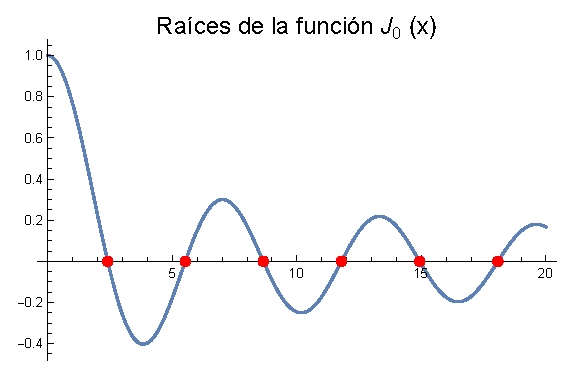
\includegraphics[scale=1]{Imagenes/Plot_Bessel_Cadena_01_Raices_J0.eps}
\end{figure}
\end{frame}
\begin{frame}
\frametitle{Modos normales de oscilación}
Los modos normales de la cadena colgante son:
\pause
\begin{align}
y_{n} (x) = J_{0} \bigg( z_{n} \, \sqrt{\dfrac{x}{L}} \bigg)
\label{eq:ecuacion_28}
\end{align}
\end{frame}
\begin{frame}
\frametitle{Oscilación de la cadena}
Con la raíz $z_{1}$:
\begin{figure}[H]
    \centering
    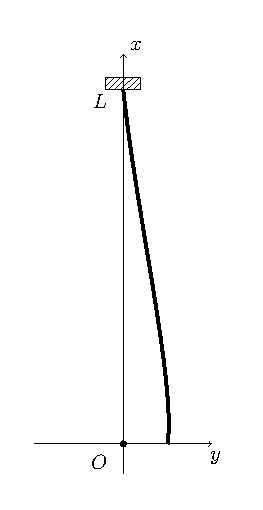
\includegraphics[scale=0.75]{Imagenes/Cadena_Oscilante_03.eps}
\end{figure}
\end{frame}
\begin{frame}
\frametitle{Oscilación de la cadena}
Con la raíz $z_{2}$:
\begin{figure}[H]
    \centering
    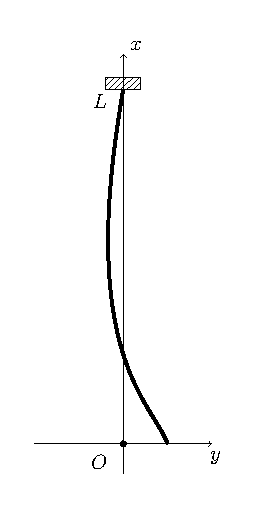
\includegraphics[scale=0.75]{Imagenes/Cadena_Oscilante_04.eps}
\end{figure}
\end{frame}
% \begin{figure}[H]
%     \centering
%     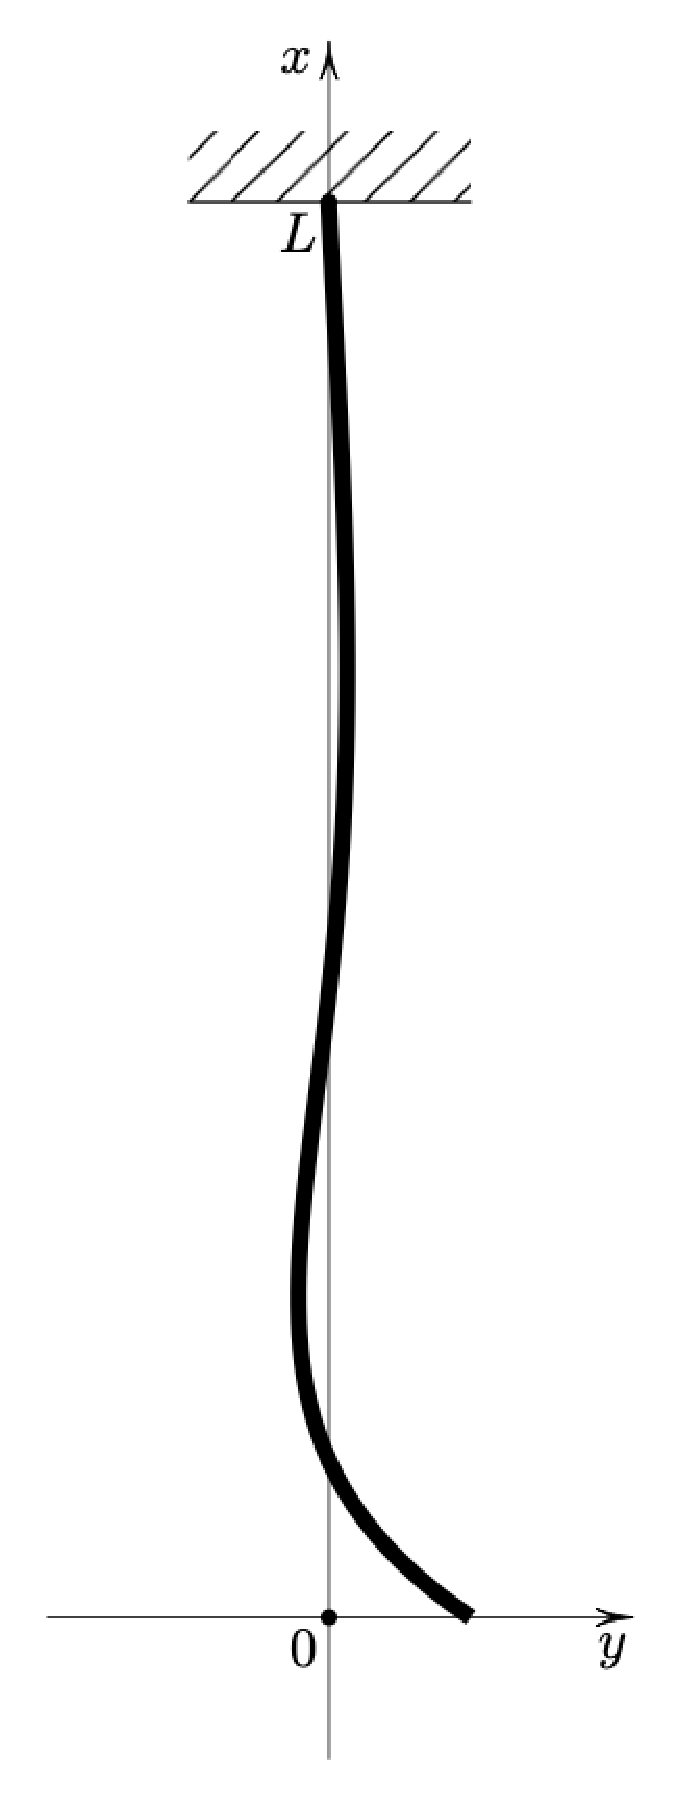
\includegraphics[scale=0.5]{Imagenes/Cadena_Oscilante_05_png.eps}
% \end{figure}

\end{document}